\section{消息认证码的定义}\label{sec:6-1}

我们首先定义什么是基于发送方和接收方之间共享密钥的消息完整性系统。由于历史原因,这种系统被称为\textbf{消息认证码 (Message Authentication Code, MAC)}。

\begin{definition}\label{def:6-1}
一个 \textbf{MAC} 系统 $\mathcal{I}=(S,V)$ 是一对有效算法 $S$ 和 $V$,其中 $S$ 称为\textbf{签名算法 (signing algorithm)},$V$ 称为\textbf{验证算法 (verification algorithm)}。算法 $S$ 用于生成标签,算法 $V$ 用于验证标签。
\begin{itemize}
	\item $S$ 是一个概率性算法,其调用方式为 $t\overset{\rm R}\leftarrow S(k,m)$,其中 $k$ 是一个密钥,$m$ 是一条消息,输出 $t$ 称为\textbf{标签 (tag)}。
	\item $V$ 是一个确定性算法,其调用方式为 $r\leftarrow V(k,m,t)$,其中 $k$ 是一个密钥,$m$ 是一条消息,$t$ 是一个标签,输出 $r$ 是 $\mathsf{accept}$ 或者 $\mathsf{reject}$。
	\item 我们要求,由 $S$ 生成的标签总是会被 $V$ 接受;也就是说,MAC 必须满足以下\textbf{正确性属性 (correctness property)}:对于所有密钥 $k$ 和所有消息 $m$,都有:
\end{itemize}
\[
\Pr\left[V\big(k,\,m,\,S(k,m)\big)=\mathsf{accept}\right]=1
\]
和之前一样,我们说密钥位于某个有限的\textbf{密钥空间} $\mathcal{K}$ 中,消息位于一个有限的\textbf{消息空间} $\mathcal{M}$ 中,标签位于某个有限的\textbf{标签空间} $\mathcal{T}$ 中。我们称 $\mathcal{I}=(S,V)$ 定义在 $(\mathcal{K},\mathcal{M},\mathcal{T})$ 上。
\end{definition}

图 \ref{fig:6-1} 展示了算法 $S$ 和算法 $V$ 是如何保护双方的网络通信的。每当算法 $V$ 对某个消息-标签对 $(m,t)$ 输出 $\mathsf{accept}$ 时,我们就称 $t$ 是 $m$ 在密钥 $k$ 下的\textbf{有效标签 (valid tag)},或者说 $(m,t)$ 是 $k$ 下的\textbf{有效对 (valid pair)}。自然,我们希望 MAC 系统中的标签尽可能短,以使得传输标签的开销最小。

在本章中,我们将探索各种 MAC 系统。在最简单的 MAC 系统中,签名算法 $S$ 是确定性的,而验证算法的定义为:
\[
V(k,m,t)=\left\{
\begin{array}{ll}
\mathsf{accept}, & S(k,m)=t\\
\mathsf{reject}, & \text{otherwise}
\end{array}
\right.
\]
我们称这样的 MAC 系统为\textbf{确定性 MAC 系统}。确定性 MAC 系统的一个属性是它有\textbf{唯一标签 (unique tags)},即对于一个给定的密钥 $k$ 和一条给定的消息 $m$,该系统在 $k$ 下对 $m$ 有一个唯一的有效标签。不是所有的 MAC 系统都有这样简单的设计,有些可能会有随机的签名算法,所以对于给定的密钥 $k$ 和消息 $m$,$S(k,m)$ 的输出可能是许多可能的有效标签中的一个,而验证算法会以其他方式工作。正如我们将看到的,这种\textbf{随机化 MAC 系统}不是实现安全的必要条件,但它们可以产生更好的效率/安全权衡。

\begin{snote}[安全的 MAC。]
接下来,我们尝试描述一个 MAC 系统的安全性到底意味着什么。为了构建在各种应用中都能保持安全的 MAC,我们将坚持在一个非常恶劣的环境中定义安全性。由于大多数现实世界中使用 MAC 的系统都运行在不太恶劣的环境中,因此我们保守的安全定义将能够保证所有系统的安全性。

我们首先直观地解释这个定义,然后说明为什么这个保守的定义是有意义的。假设一个对手正在攻击一个 MAC 系统 $\mathcal{I}=(S,V)$。令 $k$ 是某个随机选出的 MAC 密钥,它对攻击者是未知的。我们允许攻击者为其选出的任意消息 $m$ 请求标签 $t:=S(k,m)$。这种攻击被称为\textbf{选择消息攻击 (chosen message attack)},它让攻击者能够收集到数以百万计的有效消息-标签对。显然,我们给了攻击者相当大的权力——很难想象一个用户会蠢到签署由攻击者提供的任意消息。然而,我们将看到,在现实世界的环境下,选择消息攻击时有出现。我们把对手使用选择消息攻击获得的信息-标签对 $(m,t)$ 称为\textbf{签名对 (signed pair)}。

使用选择消息攻击,我们要求攻击者给出一个\textbf{存在性 MAC 伪造 (existential MAC forgery)}。也就是说,攻击者只需要想出一些\emph{新的}有效信息-标签对 $(m,t)$。所谓``新",我们指的是与所有已有签名对都不同的消息-标签对。攻击者可以自由地选择 $m$;事实上,$m$ 不需要有任何特殊的格式或意义,甚至完全可以是胡言乱语。

如果一个能够发动选择消息攻击的对手也不能创造一个存在性 MAC 伪造,我们就称这个 MAC 系统是安全的。这个定义给对手的权力和空间比它在现实场景中能得到的要多得多,而且我们要求它做的也都是一些看起来没什么意义的事情;为一个没有意义的消息伪造 MAC 似乎是没有什么用处的。然而,正如我们将要看到的,这种保守的定义是非常自然的,它使我们能够将 MAC 用于许多不同的应用。

我们使用挑战者和对手 $\mathcal{A}$ 之间的一个攻击游戏来精确地定义一个安全的 MAC。下面的文字描述和图 \ref{fig:6-2} 共同刻画了这个攻击游戏。
\end{snote}

\begin{game}[MAC 的安全性]\label{game:6-1}
对于定义在 $(\mathcal{K},\mathcal{M},\mathcal{T})$ 上一个给定的 MAC 系统 $\mathcal{I}=(S,V)$,以及一个给定的对手 $\mathcal{A}$,攻击游戏运行如下:
\begin{itemize}
	\item 挑战者随机选取 $k\overset{\rm R}\leftarrow\mathcal{K}$。
	\item $\mathcal{A}$ 向挑战者发起多次查询。\\
	对于 $i=1,2,\dots$,第 $i$ 次\emph{签名查询}是一条消息 $m_i\in\mathcal{M}$。\\
	给定 $m_i$,挑战者计算出一个标签 $t_i\overset{\rm R}\leftarrow S(k,m_i)$,然后将 $t_i$ 交给 $\mathcal{A}$。
	\item 最终,$\mathcal{A}$ 输出一个不在签名对中的候选伪造对 $(m,t)\in\mathcal{M}\times\mathcal{T}$,即:
	\[(m,t)\notin\{(m_1,t_1),(m_2,t_2),\dots\}\]
\end{itemize}
如果 $(m,t)$ 是 $k$ 下的一个有效对(即 $V(k,m,t)=\mathsf{accept}$),我们就说 $\mathcal{A}$ 赢得了上述游戏。我们将 $\mathcal{A}$ 就 $\mathcal{I}$ 的优势表示为 ${\rm MAC}\mathsf{adv}[\mathcal{A},\mathcal{I}]$,即 $\mathcal{A}$ 赢得该游戏的概率。最后,如果 $\mathcal{A}$ 最多能够发起 $Q$ 次签名查询,我们就称 $\mathcal{A}$ 是一个 \textbf{$Q$ 次查询 MAC 对手}。
\end{game}

\begin{figure}
  \centering
%  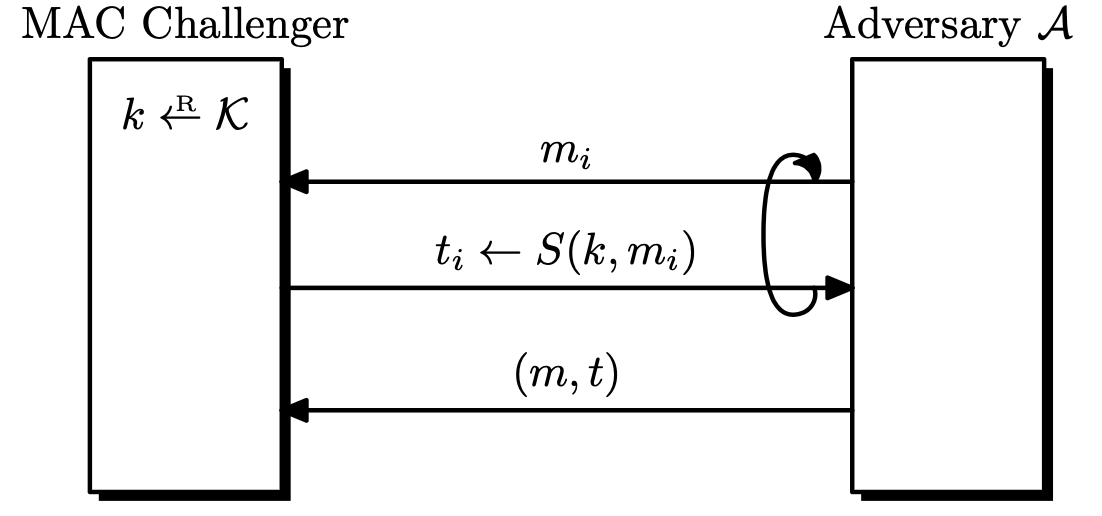
\includegraphics[width=0.5\linewidth]{figures/chapter6/fig2.png}
  \tikzset{every picture/.style={line width=0.75pt}} %set default line width to 0.75pt        

\begin{tikzpicture}[x=0.75pt,y=0.75pt,yscale=-1,xscale=1]
%uncomment if require: \path (0,195); %set diagram left start at 0, and has height of 195

%Shape: Rectangle [id:dp9400994371079527] 
\draw  [fill={rgb, 255:red, 255; green, 255; blue, 255 }  ,fill opacity=1 ][line width=1.2] [general shadow={fill=black,shadow xshift=2.25pt,shadow yshift=-2.25pt}] (30,30) -- (90,30) -- (90,180) -- (30,180) -- cycle ;
%Shape: Rectangle [id:dp23634228156893733] 
\draw  [fill={rgb, 255:red, 255; green, 255; blue, 255 }  ,fill opacity=1 ][line width=1.2] [general shadow={fill=black,shadow xshift=2.25pt,shadow yshift=-2.25pt}] (240,30) -- (300,30) -- (300,180) -- (240,180) -- cycle ;
%Straight Lines [id:da4832307524101793] 
\draw    (90,105) -- (237,105) ;
\draw [shift={(240,105)}, rotate = 180] [fill={rgb, 255:red, 0; green, 0; blue, 0 }  ][line width=0.08]  [draw opacity=0] (7.14,-3.43) -- (0,0) -- (7.14,3.43) -- cycle    ;
%Straight Lines [id:da49095779638687986] 
\draw    (95,140) -- (240,140) ;
\draw [shift={(92,140)}, rotate = 0] [fill={rgb, 255:red, 0; green, 0; blue, 0 }  ][line width=0.08]  [draw opacity=0] (7.14,-3.43) -- (0,0) -- (7.14,3.43) -- cycle    ;
%Straight Lines [id:da8544643220431498] 
\draw    (95,70) -- (240,70) ;
\draw [shift={(92,70)}, rotate = 0] [fill={rgb, 255:red, 0; green, 0; blue, 0 }  ][line width=0.08]  [draw opacity=0] (7.14,-3.43) -- (0,0) -- (7.14,3.43) -- cycle    ;
%Shape: Arc [id:dp898260212196978] 
\draw  [draw opacity=0] (231.07,104.86) .. controls (229.39,108.09) and (227.28,110) .. (225,110) .. controls (219.48,110) and (215,98.81) .. (215,85) .. controls (215,71.19) and (219.48,60) .. (225,60) .. controls (228.19,60) and (231.04,63.74) .. (232.87,69.56) -- (225,85) -- cycle ; \draw    (231.07,104.86) .. controls (229.39,108.09) and (227.28,110) .. (225,110) .. controls (219.48,110) and (215,98.81) .. (215,85) .. controls (215,71.19) and (219.48,60) .. (225,60) .. controls (227.65,60) and (230.06,62.58) .. (231.85,66.78) ; \draw [shift={(232.87,69.56)}, rotate = 245.45] [fill={rgb, 255:red, 0; green, 0; blue, 0 }  ][line width=0.08]  [draw opacity=0] (7.14,-3.43) -- (0,0) -- (7.14,3.43) -- cycle    ; 

% Text Node
\draw (60,45) node    {$k\overset{\mathrm{R}}{\leftarrow }\mathcal{K}$};
% Text Node
\draw (60,15) node   [align=left] {MAC 挑战者};
% Text Node
\draw (270,15) node   [align=left] {对手 $\displaystyle \mathcal{A}$};
% Text Node
\draw (166,66.6) node [anchor=south] [inner sep=0.75pt]    {$m_{i}$};
% Text Node
\draw (165,101.6) node [anchor=south] [inner sep=0.75pt]    {$t_{i}\leftarrow S( k,m_{i})$};
% Text Node
\draw (166,136.6) node [anchor=south] [inner sep=0.75pt]    {$( m,t)$};


\end{tikzpicture}
  \caption{MAC 攻击游戏(攻击游戏 \ref{game:6-1})}
  \label{fig:6-2}
\end{figure}

\begin{definition}\label{def:6-2}
如果对于所有有效对手 $\mathcal{A}$,${\rm MAC}\mathsf{adv}[\mathcal{A},\mathcal{I}]$ 的值都可忽略不计,我们就称 MAC 系统 $\mathcal{I}$ 是安全的。
\end{definition}

在对手赢得攻击游戏 \ref{game:6-1} 的情况下,它发送给挑战者的数对 $(m,t)$ 被称为\textbf{存在性伪造 (existential forgery)}。如果一个 MAC 系统满足定义 \ref{def:6-2},我们就称其在选择消息攻击下是\textbf{存在性不可伪造 (existential unforgeable)} 的。

在确定性 MAC 系统的情况下,$\mathcal{A}$ 赢得攻击游戏 \ref{game:6-1} 的唯一方法是为某个新消息 $m\notin\{m_1,m_2,\dots\}$  产生一个有效的消息-标签对 $(m,t)$。事实上,这种情况下的安全性只是意味着 $S$ 是\emph{不可预测的},参见 \ref{subsec:4-1-1} 小节给出的定义;也就是说,给定 $S(k,m_1),S(k,m_2),\dots$,对于任何 $m\notin\{m_1,m_2,\dots\}$,预测出 $S(k,m)$ 都是很难的。

在概率性 MAC 系统的情况下,我们的安全定义抓住了一个更强的属性。对于一条给定的消息,可能有许多条有效的标签。假设 $m$ 是某一条消息,又假设对手请求了 $m$ 的一条或多条有效标签 $t_1,t_2,\dots$,那么对手能否为 $m$ 产生一条新的有效标签 $t'$?(即一个满足 $t'\notin\{t_1,t_2,\dots\}$ 的标签)。我们的定义表明,对于一个有效对 $(m,t')$,如果 $t'$ 是新的,它就是一个有效的存在性伪造。因此,为了使 MAC 是安全的,对手必须很难为先前已经签署的消息 $m$ 产生一个新的有效标签 $t'$,这个对 MAC 的要求似乎很奇怪。如果对手已经有了 $m$ 的有效标签,我们为什么还要关心它是否能产生另一个呢?正如我们将要在第\ref{chap:9}章看到的,我们的安全定义,即防止对手在已签名的消息上产生新的标签,对于我们所考虑的应用是必要的。

回顾一下引言中的两个例子,我们可以发现,存在性不可伪造性意味着攻击者不能用一个有效标签来创建一条假的新闻报道。同样地,攻击者不能在篡改磁盘上程序的同时还不使程序的标签无效。但是,请注意,当使用 MAC 来保护应用程序的代码时,用户必须在每次要运行应用程序时提供他们的 MAC 密钥,这是一个很烦人的事情。在第\ref{chap:8}章,我们会讨论一种可以保护公共应用程序代码的无密钥方法。

为了深化对安全 MAC 的理解,我们不妨看几个案例。令 $\mathcal{I}=(S,V)$ 是一个定义在 $(\mathcal{K},\mathcal{M},\mathcal{T})$ 上的 MAC,令 $k$ 是 $\mathcal{K}$ 上的一个随机密钥。

\begin{example}\label{exmp:6-3}
假设 $m_1$ 和 $m_2$ 是几乎相同的两条消息。比如,$m_1$ 是一张 $100$ 美元的汇款单,而 $m_2$ 是一张 $101$ 美元的汇款单。显然,一个截获了 $m_1$ 的有效标签的对手不应当能够从中推导出$m_2$ 的有效标签。一个满足定义 \ref{def:6-2} 的 MAC 系统可以确保这一点。为了了解原因,假设一个对手 $\mathcal{A}$ 能够在给定 $m_1$ 的标签的情况下伪造 $m_2$ 的标签。那么,$\mathcal{A}$ 就可以赢得攻击游戏 \ref{game:6-1},方法是使用选择消息攻击来请求 $m_1$ 的标签,然后据此推导出 $m_2$ 的伪造标签 $t_2$,并输出 $(m_2,t_2)$ 作为有效的存在性伪造。显然,$\mathcal{A}$ 赢得了攻击游戏 \ref{game:6-1}。因此,存在性不可伪造性抓住了这样一个事实,即消息 $m_1$ 的标签对于产生另一条消息 $m_2$ 的标签来说不会提供任何有用的信息,即使 $m_2$ 和 $m_1$ 是几乎相同的。
\end{example}

\begin{example}\label{exmp:6-4}
我们对安全的 MAC 的定义使对手有能力获得任意消息的标签,这似乎是给了对手太多的权力。然而,在实践中,许多情况下,选择消息攻击是可行的。原因是 MAC 签名者往往不知道被签名数据的来源。例如,考虑一个将磁盘内容转储到备份磁带上的备份系统。由于备份的完整性是很重要的,系统为每一个将要被写入磁带的磁盘分组计算出一个完整性标签。该标签与数据分组一起被存储到磁带上。现在,假设一个攻击者将数据写到磁盘的低安全性区域。攻击者的数据将被备份,系统将对其计算出一个标签。通过检查所生成的备份磁带,攻击者就能获得它所选择的消息的标签。如果 MAC 系统对选择消息攻击是安全的,那么这种操作并不能帮助攻击者破解系统。
\end{example}

\begin{remark}\label{remark:6-1}
就像我们对其他安全原语所做的那样,我们可以把安全的 MAC 的概念推广到多密钥设置中,并证明一个安全的 MAC 在多密钥设置中也是安全的。参见练习 \ref{exer:6-3}。
\end{remark}

\subsection{数学细节}

和之前一样,我们使用 \ref{sec:2-3} 节中定义的术语,对 MAC 给出一个更精确的数学定义。读者在初读时可以安全地跳过这一小节。

\begin{definition}[MAC]\label{def:6-3}
一个 \textbf{MAC} 系统是一对有效算法 $S$ 和 $V$,以及三个具有系统参数化 $P$ 的空间族:
\[
\mathbf{K}=\{\mathcal{K}_{\lambda,\Lambda}\}_{\lambda,\Lambda},\quad
\mathbf{M}=\{\mathcal{M}_{\lambda,\Lambda}\}_{\lambda,\Lambda},\quad
\mathbf{T}=\{\mathcal{T}_{\lambda,\Lambda}\}_{\lambda,\Lambda}
\]
和之前一样,$\lambda\in Z_{\geq1}$ 是一个安全参数,$\Lambda\in{\rm Supp}(P(\lambda))$ 是一个领域参数。我们要求:
\begin{enumerate}
	\item $\mathbf{K}$,$\mathbf{M}$ 和 $\mathbf{T}$ 是可有效识别的。
	\item $\mathbf{K}$ 是可有效采样的。
	\item 算法 $S$ 是一个有效的概率性算法,对于输入 $\lambda\in\mathbb{Z}_{\geq1}$,$\Lambda\in{\rm Supp}(P(\lambda))$,$k\in\mathcal{K}_{\lambda,\Lambda}$ 和 $m\in\mathcal{M}_{\lambda,\Lambda}$,$S$ 输出 $\mathcal{T}_{\lambda,\Lambda}$ 中的一个元素。
	\item 算法 $V$ 是一个有效确定性算法,对于输入 $\lambda\in\mathbb{Z}_{\geq1}$,$\Lambda\in{\rm Supp}(P(\lambda))$,$k\in\mathcal{K}_{\lambda,\Lambda}$,$m\in\mathcal{M}_{\lambda,\Lambda}$ 和 $t\in\mathcal{T}_{\lambda,\Lambda}$,$V$ 输出 $\mathsf{accept}$ 或 $\mathsf{reject}$。
\end{enumerate}

\end{definition}

在定义安全性时,我们通过安全参数 $\lambda$ 将攻击游戏 \ref{game:6-1} 参数化,对手和挑战者都会得到该参数。因此,优势 ${\rm MAC}\mathsf{adv}[\mathcal{A},\mathcal{I}]$ 也是 $\lambda$ 的一个函数。定义 \ref{def:6-2} 应该被理解为 ${\rm MAC}\mathsf{adv}[\mathcal{A},\mathcal{I}](\lambda)$ 是一个可忽略不计函数。